% VAMOS Paper: IEEE Transactions on Evolutionary Computation (IEEE TEVC)
% =============================================================================
% Supplementary Material
% =============================================================================
\documentclass[journal]{IEEEtran}

\usepackage{cite}
\usepackage{graphicx}
\usepackage{booktabs}
\usepackage{amsmath}
\usepackage{amssymb}
\usepackage{multirow}
\usepackage{algorithm}
\usepackage{algpseudocode}
\usepackage{listings}
\usepackage{xcolor}
\usepackage{pifont}
\usepackage{enumitem}
\usepackage{stfloats}
\newcommand{\cmark}{\ding{51}}
\newcommand{\pmark}{\ding{109}}
\newcommand{\xmark}{\ding{55}}
\usepackage[hidelinks]{hyperref}
\hypersetup{hypertexnames=false}
\makeatletter
\g@addto@macro\UrlBreaks{\do\.\do\_\do\-\do\/}
\makeatother

% Code listing style
\lstset{
  language=Python,
  basicstyle=\ttfamily\scriptsize,
  keywordstyle=\bfseries\color{green!50!black},
  commentstyle=\itshape\color{teal},
  stringstyle=\color{red!70!black},
  identifierstyle=\color{black},
  showstringspaces=false,
  frame=lines,
  rulecolor=\color{gray!20},
  breaklines=true,
  numbers=left,
  numbersep=5pt,
  numberstyle=\tiny\color{black},
  captionpos=b,
  xleftmargin=.5em,
  framexleftmargin=.5em,
  aboveskip=.5em,
  belowskip=.5em
}

\renewcommand{\lstlistingname}{Code}% Listing -> Code

\newcommand{\VAMOS}{VAMOS}
\newcommand{\HV}{\mathrm{HV}}
\newcommand{\Intdomain}[1]{[#1]_{\mathbb{Z}}}
\newcommand{\Realdomain}[1]{[#1]_{\mathbb{R}}}

\title{VAMOS: A Framework for Fast, Configurable and Accessible Multiobjective Optimization in Python\\\vspace{3mm}\Large{(Supplementary Material)}}

% --------------------------------------------------------------------------
%  Author block.
% --------------------------------------------------------------------------
%\author{Nicol\'{a}s~R.~Uribe,
%        Alberto~Herr\'{a}n,
%        Antonio~J.~Nebro,
%        Javier~Del~Ser,
%        and~J.~Manuel~Colmenar%
%\thanks{N. R. Uribe, A. Herr\'{a}n, and J. M. Colmenar are with the
%  Department of Computer Sciences, Universidad Rey Juan Carlos, M\'{o}stoles,
%  28933 Madrid, Spain (e-mail: nicolas.rodriguez@urjc.es; alberto.herran@urjc.es;
%  josemanuel.colmenar@urjc.es).}%
%\thanks{A. J. Nebro is with the Department of Lenguajes y Ciencias de la
%  Computaci\'{o}n, ITIS Software, University of M\'{a}laga, 29071
%  M\'{a}laga, Spain (e-mail: ajnebro@uma.es).}%
%\thanks{J. Del Ser is with TECNALIA, Basque Research \& Technology
%  Alliance (BRTA), Derio, 48160, Spain, and also with the University
%  of the Basque Country (UPV/EHU), Leioa, 48940, Spain (e-mail: javier.delser@tecnalia.com).}%
%\thanks{Corresponding author: Nicol\'{a}s~Rodr\'{i}guez (nicolas.rodriguez@urjc.es).}%
%}
\author{Anonymous submission}

\markboth{IEEE Transactions on Evolutionary Computation}%
{A Vectorized Framework for Multiobjective Evolutionary Optimization}

\begin{document}
\maketitle

This Supplementary Material accompanies the main manuscript and contains the extended convergence, solution-quality, runtime, statistical, configurability, and accessibility results referenced there.

%==============================================================================
\section{Convergence Analysis}
\label{app:convergence}
%==============================================================================

\begin{figure*}[!t]
  \centering
  
\includegraphics[width=\textwidth]{convergence.png}
  \caption{Convergence of normalized hypervolume over 50{,}000 evaluations for \VAMOS{} (Numba), \textit{pymoo} , and \textit{jMetalPy} on DTLZ2 (3 objectives, 12 variables), WFG4 (2 objectives, 24 variables), and ZDT1 (2 objectives, 30 variables). Solid/dashed lines show median hypervolume values across 30 seeds; shaded regions indicate the interquartile range. All three frameworks follow nearly identical convergence trajectories, confirming that the semantic alignment protocol produces equivalent algorithmic behavior.}
  \label{fig:convergence}
\end{figure*}

To verify that runtime speedups do not come at the expense of convergence rate, we track normalized hypervolume at 1{,}000-evaluation intervals over the full 50{,}000-evaluation budget. Fig.~\ref{fig:convergence} compares \VAMOS{}, \textit{pymoo} , and \textit{jMetalPy} on three representative problems: DTLZ2 (3 objectives, 12 variables), WFG4 (2 objectives, 24 variables), and ZDT1 (2 objectives, 30 variables). The convergence curves are nearly indistinguishable across all three frameworks, with overlapping interquartile ranges across all 30 seeds. All frameworks reach the same final quality at the same evaluation counts, confirming that the performance gains observed in runtime measurements are not accompanied by degraded convergence behavior.


%==============================================================================
\section{Solution Quality Analysis}
\label{app:quality}
%==============================================================================
The runtime advantages reported above are only meaningful if \VAMOS{} produces solutions of comparable quality. To verify this, we compare normalized hypervolume (HV) across frameworks using the protocol described in Section~V-E of the main paper: for each problem we compute the median HV across 30 seeds, and then summarize these per-problem medians by family using the median and interquartile range (IQR). Table~\ref{tab:frameworks_hv} presents the results for the generational Non-dominated Sorting Genetic Algorithm II (NSGA-II).

\begin{table*}[htbp]
\centering
%\scriptsize
%\setlength{\tabcolsep}{3pt}
\caption{Normalized hypervolume summary (median (IQR)) by problem family across frameworks}
\label{tab:frameworks_hv}
\begin{tabular}{@{}lccccc@{}}
\toprule
\textbf{Framework} & \textbf{ZDT} & \textbf{DTLZ} & \textbf{WFG} & \textbf{ZCAT} & \textbf{Overall} \\
\midrule
VAMOS & \textbf{0.991 (0.013)} & 0.836 (0.121) & \textbf{0.934 (0.138)} & --- & \textbf{0.934 (0.157)} \\
\textit{pymoo} & \textbf{0.991 (0.010)} & 0.829 (0.148) & 0.846 (0.220) & --- & 0.921 (0.156) \\
\textit{jMetalPy} & \textbf{0.991 (0.014)} & 0.835 (0.110) & 0.845 (0.223) & --- & 0.924 (0.159) \\
\textit{DEAP} & \textbf{0.991 (0.013)} & \textbf{0.839 (0.138)} & 0.839 (0.224) & --- & 0.924 (0.156) \\
\textit{Platypus} & \textbf{0.991 (0.010)} & 0.824 (0.177) & 0.919 (0.137) & --- & 0.919 (0.160) \\
\bottomrule
\end{tabular}
\end{table*}

Across ZDT, all frameworks attain nearly identical normalized HV, confirming that benchmark definitions and operator semantics are effectively aligned. For DTLZ, medians are tightly clustered across frameworks. WFG exhibits the largest dispersion; notably, \VAMOS{} achieves the highest median on WFG (0.934 vs.\ 0.846 for \textit{pymoo} ), which may reflect subtle differences in WFG parameterization or boundary handling across implementations. Together with the runtime results, these summaries confirm that \VAMOS{} achieves comparable or superior solution quality while delivering faster runtimes under the fixed-reference-front protocol.

Table~\ref{tab:frameworks_hv_variants} extends this analysis to the NSGA-II steady-state and external-archive variants. For the steady-state variant, the overall normalized HV is effectively identical across frameworks (all three reach 0.989 overall), although \VAMOS{} attains a clearly higher median on WFG (0.939 vs.\ 0.849 for \textit{pymoo}  and 0.848 for jMetalPy). For the archive variant, the three frameworks remain closely matched across all families: ZDT and ZCAT are virtually identical, DTLZ differs by at most 0.003, and the WFG medians lie in the narrow 0.846--0.852 range.

\begin{table*}[htbp]
\centering
%\scriptsize
%\setlength{\tabcolsep}{3pt}
\caption{Normalized hypervolume summary (median (IQR)) by problem family for NSGA-II variants}
\label{tab:frameworks_hv_variants}
\begin{tabular}{@{}llccccc@{}}
\toprule
\textbf{Algorithm} & \textbf{Framework} & \textbf{ZDT} & \textbf{DTLZ} & \textbf{WFG} & \textbf{ZCAT} & \textbf{Overall} \\
\midrule
NSGA-II (SS) & VAMOS & 0.993 (0.009) & 0.846 (0.091) & 0.939 (0.138) & 0.994 (0.004) & 0.989 (0.055) \\
 & \textit{pymoo}  & 0.993 (0.008) & 0.847 (0.160) & 0.849 (0.218) & 0.994 (0.004) & 0.989 (0.073) \\
 & \textit{jMetalPy} & 0.993 (0.009) & 0.849 (0.101) & 0.848 (0.153) & 0.994 (0.004) & 0.989 (0.073) \\
\midrule
NSGA-II (Archive) & VAMOS & 0.993 (0.010) & 0.855 (0.106) & 0.846 (0.219) & 0.993 (0.005) & 0.987 (0.079) \\
 & \textit{pymoo}  & 0.993 (0.009) & 0.853 (0.139) & 0.852 (0.223) & 0.993 (0.005) & 0.988 (0.080) \\
 & \textit{jMetalPy} & 0.993 (0.010) & 0.856 (0.104) & 0.846 (0.149) & 0.993 (0.005) & 0.987 (0.073) \\
\bottomrule
\end{tabular}
\end{table*}

%% Auto-generated by 16_update_igd_tables_from_csv.py

\begin{table*}[htbp]
\centering
\caption{IGD+ summary (median (IQR)) by problem family across frameworks and algorithms. Lower values indicate closer proximity to the reference Pareto front}
\label{tab:frameworks_igd_merged}
\begin{tabular}{llccccc}
\toprule
\textbf{Algorithm} & \textbf{Framework} & \textbf{ZDT} & \textbf{DTLZ} & \textbf{WFG} & \textbf{ZCAT} & \textbf{Overall\textsuperscript{*}} \\
\midrule
NSGA-II & VAMOS & 0.0030 (0.0016) & 0.0357 (0.0172) & 0.0699 (0.1257) & 0.0050 (0.0016) & 0.0059 (0.0310) \\
 & pymoo & 0.0024 (0.0015) & 0.0351 (0.0269) & 0.0700 (0.1294) & 0.0049 (0.0016) & 0.0059 (0.0309) \\
 & jMetalPy & 0.0030 (0.0015) & 0.0351 (0.0175) & 0.0699 (0.1287) & 0.0049 (0.0016) & 0.0059 (0.0306) \\
 & DEAP & 0.0029 (0.0015) & 0.0349 (0.0243) & 0.0690 (0.1318) & 0.0049 (0.0016) & 0.0059 (0.0301) \\
 & Platypus & 0.0023 (0.0014) & 0.0352 (0.0224) & 0.0576 (0.1131) & 0.0053 (0.0015) & 0.0061 (0.0307) \\
\midrule
SMS-EMOA & VAMOS & 0.0019 (0.0012) & 0.0219 (0.0333) & 0.0578 (0.1293) & 0.0027 (0.0009) & 0.0032 (0.0161) \\
 & pymoo & 0.0019 (0.0012) & 0.0185 (0.0078) & 0.0552 (0.1273) & 0.0027 (0.0009) & 0.0032 (0.0161) \\
 & jMetalPy & 0.0019 (0.0012) & 0.0220 (0.0319) & 0.0569 (0.1289) & 0.0027 (0.0009) & 0.0032 (0.0161) \\
\midrule
MOEA/D & VAMOS & 0.0025 (0.0002) & 0.0345 (0.0271) & 0.0694 (0.1211) & 0.0065 (0.0006) & 0.0067 (0.0273) \\
 & pymoo & 0.0025 (0.0001) & 0.0396 (0.0480) & 0.0682 (0.1184) & 0.0066 (0.0006) & 0.0068 (0.0283) \\
 & jMetalPy & 0.0025 (0.0002) & 0.0347 (0.0287) & 0.0682 (0.1189) & 0.0065 (0.0006) & 0.0067 (0.0272) \\
 & Platypus & --- & --- & --- & 0.0066 (0.0006) & 0.0066 (0.0006) \\
\bottomrule
\end{tabular}
\end{table*}


%==============================================================================
\section{Statistical Analysis}
\label{app:stats_main}
%==============================================================================

The descriptive summaries in the previous section suggest quality equivalence, but median and IQR alone cannot determine whether observed differences are statistically significant. We therefore apply Wilcoxon signed-rank tests (paired by seed) comparing \VAMOS{} against each competitor on every problem, with Holm step-down correction for familywise error control ($\alpha=0.05$). As a measure of practical significance, we report the Vargha--Delaney $\hat{A}_{12}$ effect size~\cite{VD00} alongside each test ($\hat{A}_{12}>0.5$ favors \VAMOS{}; thresholds: negligible${}<0.56$, small${}<0.64$, medium${}<0.71$, large${\ge}0.71$). We also compute paired-bootstrap 90\% confidence intervals (CIs) for the relative normalized-HV difference $\Delta = (\HV_{\text{VAMOS}} - \HV_{\text{fw}})/\HV_{\text{fw}}$, and declare \emph{equivalence} when the entire CI falls within $\pm 1\%$.

Table~\ref{tab:stats_hypervolume_nsgaii} presents the per-problem Wilcoxon results for the NSGA-II baseline. Of 41 problems, only one (ZDT6) shows a statistically significant difference in normalized HV after Holm correction, and the magnitude is small ($\Delta \approx 0.4\%$). Table~\ref{tab:hv_equivalence_summary_nsgaii} summarizes the equivalence analysis: \VAMOS{} is equivalent to \textit{pymoo}  on 37/41 problems and non-inferior on 38/41, with a median $\Delta$HV of $-0.01\%$. Similar patterns hold for \textit{jMetalPy} and the other frameworks. Table~\ref{tab:hv_robustness_summary_nsgaii} details robustness, and Fig.~\ref{fig:forest_ci_nsgaii} visualizes per-problem CIs as a forest plot. Detailed NSGA-II statistical tables are provided in Section~\ref{app:stats_nsgaii}, and corresponding analyses for SMS-EMOA and MOEA/D are provided in Section~\ref{app:stats}.

%==============================================================================
\section{Additional runtime comparisons}
\label{app:variants}
%==============================================================================
This section reports supplementary runtime comparisons for NSGA-II variants (steady-state and external archive), the S-metric Selection Evolutionary Multiobjective Optimization Algorithm (SMS-EMOA), and the Multiobjective Evolutionary Algorithm Based on Decomposition (MOEA/D) under the same protocol as the Experimental Results section of the main paper.

\begin{table*}[htbp]
\centering
\scriptsize
\setlength{\tabcolsep}{3pt}
\caption{Median runtime (seconds) by problem family for algorithm variants}
\label{tab:frameworks_perf_variants}
\begin{tabular}{@{}llccccc@{}}
\toprule
\textbf{Algorithm} & \textbf{Framework} & \textbf{ZDT} & \textbf{DTLZ} & \textbf{WFG} & \textbf{ZCAT} & \textbf{Average} \\
\midrule
NSGA-II (SS) & VAMOS & \textbf{150.21} & \textbf{244.80} & \textbf{799.29} & \textbf{715.29} & \textbf{477.40} \\
 & \textit{pymoo}  & 5747.47 & 7259.88 & 6382.73 & 4569.01 & 5989.77 \\
 & \textit{jMetalPy} & 1930.43 & 2506.83 & 2756.07 & 1947.76 & 2285.27 \\
\midrule
NSGA-II (Arch.) & VAMOS & \textbf{10.43} & \textbf{87.56} & \textbf{23.33} & \textbf{106.30} & \textbf{56.91} \\
 & \textit{pymoo}  & 1422.71 & 7208.12 & 1515.89 & 1511.36 & 2914.52 \\
 & \textit{jMetalPy} & 744.93 & 3993.47 & 1736.74 & 602.88 & 1769.51 \\
\midrule
SMS-EMOA & VAMOS & \textbf{124.94} & \textbf{187.16} & \textbf{734.42} & \textbf{521.22} & \textbf{391.94} \\
 & \textit{pymoo}  & 1658.10 & 2439.60 & 3410.49 & 2967.14 & 2618.83 \\
 & \textit{jMetalPy} & 377.01 & 529.49 & 1161.51 & 2670.22 & 1184.56 \\
\midrule
MOEA/D & VAMOS & \textbf{76.19} & \textbf{118.98} & \textbf{647.96} & \textbf{340.78} & \textbf{295.98} \\
 & \textit{pymoo}  & 1325.29 & 1735.46 & 4143.63 & 1023.63 & 2057.00 \\
 & \textit{jMetalPy} & 303.00 & 430.14 & 4267.52 & 354.29 & 1338.74 \\
\bottomrule
\end{tabular}
\end{table*}

\subsection{Memory footprint}

Peak resident-set-size (RSS) was measured during NSGA-II runs on three representative problems (ZDT1, DTLZ2, WFG4) using 50{,}000 evaluations and 5 seeds per framework. \VAMOS{} achieves a median peak RSS of 0.28 megabytes (MB), compared to 0.84\,MB for \textit{pymoo}  ($3\times$ higher) and 0.50\,MB for \textit{jMetalPy} ($1.8\times$ higher). These measurements are consistent with the array-native representation reducing per-individual object overhead.

\begin{figure}[htbp]
\centering

\includegraphics[width=\columnwidth]{memory_comparison.png}
\caption{Peak memory footprint (MB) during NSGA-II optimization on three representative problems (50{,}000 evaluations, median of 5 seeds). \VAMOS{} consistently uses less memory than both \textit{pymoo} and \textit{jMetalPy} across the measured problems.}
\label{fig:memory_comparison}
\end{figure}

\section{Detailed statistical analysis for NSGA-II}
\label{app:stats_nsgaii}
This section reports per-problem Wilcoxon signed-rank tests, bootstrap equivalence analyses, robustness summaries, and bootstrap confidence intervals for the NSGA-II baseline discussed in the Statistical Analysis section of the main paper.
\begingroup
\setlength{\tabcolsep}{2pt}
\begin{table}[htbp]
\centering
\caption{NSGA-II. Normalized hypervolume comparison with Wilcoxon signed-rank test results (Holm-corrected)}
\label{tab:stats_hypervolume_nsgaii}
\begin{tabular}{lccccc}
\toprule
\textbf{Problem} & \textbf{VAMOS} & \textbf{pymoo} & \textbf{p-value} & \textbf{$\hat{A}_{12}$} & \textbf{Significance} \\
\midrule
dtlz1 & 0.920 & \textbf{0.921} & 1.000 & 0.47 & \xmark \\
dtlz2 & 0.826 & \textbf{0.827} & 1.000 & 0.46 & \xmark \\
dtlz3 & \textbf{0.749} & 0.673 & 0.813 & 0.66 & \xmark \\
dtlz4 & 0.828 & \textbf{0.829} & 1.000 & 0.49 & \xmark \\
dtlz5 & 0.966 & \textbf{0.966} & 1.000 & 0.45 & \xmark \\
dtlz6 & 0.444 & \textbf{0.510} & 1.000 & 0.32 & \xmark \\
dtlz7 & \textbf{0.876} & 0.874 & 1.000 & 0.53 & \xmark \\
wfg1 & 0.353 & \textbf{0.430} & 1.000 & 0.36 & \xmark \\
wfg2 & 1.007 & \textbf{1.007} & 1.000 & 0.37 & \xmark \\
wfg3 & 0.971 & \textbf{0.973} & 1.000 & 0.35 & \xmark \\
wfg4 & 0.956 & \textbf{0.957} & 1.000 & 0.48 & \xmark \\
wfg5 & 0.826 & \textbf{0.826} & 0.513 & 0.32 & \xmark \\
wfg6 & 0.840 & \textbf{0.846} & 1.000 & 0.44 & \xmark \\
wfg7 & 0.963 & \textbf{0.964} & 1.000 & 0.41 & \xmark \\
wfg8 & \textbf{0.745} & 0.745 & 1.000 & 0.54 & \xmark \\
wfg9 & 0.714 & \textbf{0.714} & 1.000 & 0.48 & \xmark \\
zcat1 & 0.983 & \textbf{0.983} & 1.000 & 0.44 & \xmark \\
zcat10 & 0.951 & \textbf{0.951} & 1.000 & 0.43 & \xmark \\
zcat11 & 0.990 & \textbf{0.990} & 1.000 & 0.48 & \xmark \\
zcat12 & 0.989 & \textbf{0.990} & 1.000 & 0.45 & \xmark \\
zcat13 & 1.016 & \textbf{1.016} & 1.000 & 0.47 & \xmark \\
zcat14 & 0.977 & \textbf{0.977} & 1.000 & 0.36 & \xmark \\
zcat15 & 0.989 & \textbf{0.990} & 1.000 & 0.45 & \xmark \\
zcat16 & 0.987 & \textbf{0.988} & 1.000 & 0.40 & \xmark \\
zcat17 & 0.995 & \textbf{0.995} & 1.000 & 0.46 & \xmark \\
zcat18 & \textbf{0.990} & 0.990 & 1.000 & 0.52 & \xmark \\
zcat19 & 0.986 & \textbf{0.986} & 1.000 & 0.42 & \xmark \\
zcat2 & 0.992 & \textbf{0.992} & 1.000 & 0.49 & \xmark \\
zcat20 & \textbf{0.990} & 0.990 & 1.000 & 0.52 & \xmark \\
zcat3 & 0.983 & \textbf{0.983} & 1.000 & 0.37 & \xmark \\
zcat4 & 0.983 & \textbf{0.983} & 1.000 & 0.37 & \xmark \\
zcat5 & 0.995 & \textbf{0.995} & 1.000 & 0.46 & \xmark \\
zcat6 & 0.995 & \textbf{0.995} & 1.000 & 0.46 & \xmark \\
zcat7 & \textbf{0.990} & 0.990 & 1.000 & 0.52 & \xmark \\
zcat8 & 0.971 & \textbf{0.971} & 1.000 & 0.49 & \xmark \\
zcat9 & 0.971 & \textbf{0.971} & 1.000 & 0.49 & \xmark \\
zdt1 & 0.991 & \textbf{0.991} & 1.000 & 0.42 & \xmark \\
zdt2 & 0.982 & \textbf{0.982} & 1.000 & 0.44 & \xmark \\
zdt3 & 0.996 & \textbf{0.996} & 1.000 & 0.55 & \xmark \\
zdt4 & 1.001 & \textbf{1.001} & 1.000 & 0.43 & \xmark \\
zdt6 & 0.982 & \textbf{0.986} & $<$0.0001 & 0.00 & \cmark \\
\bottomrule
\end{tabular}
\end{table}

\begin{table}[htbp]
\centering
\caption{NSGA-II. IGD+ comparison with Wilcoxon signed-rank test results (Holm-corrected). Lower is better}
\label{tab:stats_igd_plus_nsgaii}
\begin{tabular}{lccccc}
\toprule
\textbf{Problem} & \textbf{VAMOS} & \textbf{pymoo} & \textbf{p-value} & \textbf{$\hat{A}_{12}$} & \textbf{Significance} \\
\midrule
dtlz1 & 0.0181 & \textbf{0.0179} & 1.000 & 0.53 &  \xmark \\
dtlz2 & 0.0357 & \textbf{0.0352} & 1.000 & 0.56 &  \xmark \\
dtlz3 & \textbf{0.0518} & 0.0716 & 0.834 & 0.32 &  \xmark \\
dtlz4 & 0.0357 & \textbf{0.0351} & 1.000 & 0.54 &  \xmark \\
dtlz5 & 0.0029 & \textbf{0.0029} & 1.000 & 0.51 &  \xmark \\
dtlz6 & 0.0996 & \textbf{0.0837} & 1.000 & 0.67 &  \xmark \\
dtlz7 & 0.0350 & \textbf{0.0350} & 1.000 & 0.56 &  \xmark \\
wfg1 & 0.7451 & \textbf{0.6949} & 1.000 & 0.65 &  \xmark \\
wfg2 & 0.2162 & \textbf{0.2155} & 1.000 & 0.64 &  \xmark \\
wfg3 & 0.0206 & \textbf{0.0191} & 1.000 & 0.65 &  \xmark \\
wfg4 & 0.0133 & \textbf{0.0128} & 1.000 & 0.53 &  \xmark \\
wfg5 & \textbf{0.0699} & 0.0700 & 1.000 & 0.51 &  \xmark \\
wfg6 & 0.0600 & \textbf{0.0573} & 1.000 & 0.59 &  \xmark \\
wfg7 & 0.0106 & \textbf{0.0103} & 1.000 & 0.58 &  \xmark \\
wfg8 & \textbf{0.1463} & 0.1485 & 1.000 & 0.45 &  \xmark \\
wfg9 & \textbf{0.1263} & 0.1264 & 1.000 & 0.51 &  \xmark \\
zcat1 & 0.0074 & \textbf{0.0073} & 1.000 & 0.58 &  \xmark \\
zcat10 & 0.0033 & \textbf{0.0032} & 1.000 & 0.57 &  \xmark \\
zcat11 & 0.0049 & \textbf{0.0049} & 1.000 & 0.49 &  \xmark \\
zcat12 & 0.0050 & \textbf{0.0049} & 1.000 & 0.52 &  \xmark \\
zcat13 & 0.0038 & \textbf{0.0037} & 1.000 & 0.57 &  \xmark \\
zcat14 & 0.0070 & \textbf{0.0069} & 1.000 & 0.64 &  \xmark \\
zcat15 & 0.0050 & \textbf{0.0050} & 1.000 & 0.52 &  \xmark \\
zcat16 & 0.0048 & \textbf{0.0046} & 1.000 & 0.58 &  \xmark \\
zcat17 & 0.0040 & \textbf{0.0040} & 1.000 & 0.51 &  \xmark \\
zcat18 & \textbf{0.0044} & 0.0044 & 1.000 & 0.51 &  \xmark \\
zcat19 & 0.0062 & \textbf{0.0061} & 1.000 & 0.58 &  \xmark \\
zcat2 & 0.0059 & \textbf{0.0059} & 1.000 & 0.52 &  \xmark \\
zcat20 & \textbf{0.0045} & 0.0045 & 1.000 & 0.52 &  \xmark \\
zcat3 & 0.0074 & \textbf{0.0072} & 1.000 & 0.63 &  \xmark \\
zcat4 & 0.0074 & \textbf{0.0072} & 1.000 & 0.63 &  \xmark \\
zcat5 & 0.0040 & \textbf{0.0040} & 1.000 & 0.53 &  \xmark \\
zcat6 & 0.0027 & \textbf{0.0026} & 1.000 & 0.63 &  \xmark \\
zcat7 & \textbf{0.0044} & 0.0044 & 1.000 & 0.52 &  \xmark \\
zcat8 & 0.0057 & \textbf{0.0056} & 1.000 & 0.51 &  \xmark \\
zcat9 & 0.0057 & \textbf{0.0057} & 1.000 & 0.50 &  \xmark \\
zdt1 & 0.0032 & \textbf{0.0031} & 1.000 & 0.53 &  \xmark \\
zdt2 & 0.0030 & \textbf{0.0030} & 1.000 & 0.53 &  \xmark \\
zdt3 & \textbf{0.0015} & 0.0015 & 1.000 & 0.45 &  \xmark \\
zdt4 & 0.0008 & \textbf{0.0008} & 1.000 & 0.59 &  \xmark \\
zdt6 & 0.0031 & \textbf{0.0024} & $<$0.0001 & 1.00 & \checkmark \\
\bottomrule
\end{tabular}
\end{table}

\begin{table}[htbp]
\centering
\caption{Normalized hypervolume equivalence summary (paired bootstrap 90\% CI; equivalence margin $\pm 1\%$ relative)}
\label{tab:hv_equivalence_summary_nsgaii}
\begin{tabular}{lccc}
\toprule
\textbf{Framework} & \textbf{Eq.\ problems} & \textbf{Non-inf.\ problems} & \textbf{Median $\Delta$HV (\%)} \\
\midrule
\textit{pymoo} & 37/41 & 38/41 & -0.01 \\
\textit{jMetalPy} & 35/41 & 35/41 & -0.02 \\
\textit{DEAP} & 33/41 & 37/41 & -0.01 \\
\textit{Platypus} & 33/41 & 38/41 & +0.05 \\
\bottomrule
\end{tabular}
\end{table}

\begin{table}[htbp]
\centering
\caption{Robustness summary for normalized hypervolume across seeds (median across problems). ``Near-best'' is defined per problem as HV $\ge 0.99 \cdot \max$ median(HV) among frameworks}
\label{tab:hv_robustness_summary_nsgaii}
\begin{tabular}{lcc}
\toprule
\textbf{Framework} & \textbf{Median IQR(HV)} & \textbf{Median \% seeds near-best} \\
\midrule
VAMOS & 0.001 & 100.0 \\
\textit{pymoo} & 0.001 & 100.0 \\
\textit{jMetalPy} & 0.002 & 100.0 \\
\textit{DEAP} & 0.001 & 100.0 \\
\textit{Platypus} & 0.001 & 100.0 \\
\bottomrule
\end{tabular}
\end{table}

\begin{figure}[htbp]
  \centering
  
\includegraphics[width=\columnwidth]{forest_ci_nsgaii.png}
  \caption{NSGA-II. Per-problem paired bootstrap 90\% confidence intervals for the relative normalized hypervolume difference $\Delta = (\HV_{\text{\VAMOS}} - \HV_{\text{fw}})/\HV_{\text{fw}}$, reported in percent. The shaded band marks the $\pm 1\%$ equivalence margin; intervals falling entirely within this band indicate statistical equivalence}
  \label{fig:forest_ci_nsgaii}
\end{figure}
\endgroup

\section{Reference fronts and detailed benchmark results}
\label{app:detailed}
%==============================================================================

The repository includes dense reference Pareto fronts for all benchmark problems used for normalized hypervolume computation. These fronts are generated analytically when closed forms are available (ZDT and most DTLZ problems) and by dense sampling followed by non-dominated filtering for cases where the Pareto front is disconnected or defined implicitly (DTLZ7 and WFG). For WFG2 we use a higher sampling density to stabilize HV normalization.

Fig.~\ref{fig:runtime_heatmap} presents per-problem median runtimes as a dual-panel heatmap. The left panel compares VAMOS backends (Numba, MooCore, NumPy); the right panel compares VAMOS against \textit{pymoo}  and jMetalPy. Color intensity indicates runtime on a logarithmic scale, with annotated values in each cell and bold values marking the fastest per problem.

\begin{figure*}[htbp]
  \centering
  
\includegraphics[width=0.95\textwidth]{runtime_heatmap.png}
  \caption{Per-problem median runtime (seconds) for VAMOS backends (left) and cross-framework comparison (right). Color scale is logarithmic; bold values indicate the fastest in each row. Problems are grouped by family (ZDT, DTLZ, WFG).}
  \label{fig:runtime_heatmap}
\end{figure*}

%==============================================================================
\section{Statistical analysis for SMS-EMOA and MOEA/D}
\label{app:stats}
%==============================================================================

This section reports Wilcoxon signed-rank tests, bootstrap equivalence analyses, and robustness summaries for SMS-EMOA and MOEA/D, following the same methodology as the Statistical Analysis section of the main paper.

\subsection{SMS-EMOA}

Tables~\ref{tab:stats_hypervolume_smsemoa}--\ref{tab:hv_robustness_summary_smsemoa} present per-problem Wilcoxon tests, equivalence summaries, and robustness summaries for SMS-EMOA. Fig.~\ref{fig:forest_ci_smsemoa} visualizes per-problem bootstrap confidence intervals.

\begingroup
\setlength{\tabcolsep}{2pt}
\begin{table}[htbp]
\centering
\caption{SMS-EMOA. Normalized hypervolume comparison with Wilcoxon signed-rank test results (Holm-corrected)}
\label{tab:stats_hypervolume_smsemoa}
\begin{tabular}{lccccc}
\toprule
\textbf{Problem} & \textbf{VAMOS} & \textbf{pymoo} & \textbf{p-value} & \textbf{$\hat{A}_{12}$} & \textbf{Significance} \\
\midrule
zdt1 & 0.993 & \textbf{0.993} & 1.000 & 0.44 &  \xmark \\
zdt2 & \textbf{0.987} & 0.987 & 1.000 & 0.52 &  \xmark \\
zdt3 & 0.997 & \textbf{0.997} & 1.000 & 0.46 &  \xmark \\
zdt4 & 1.004 & \textbf{1.004} & 1.000 & 0.35 &  \xmark \\
zdt6 & \textbf{0.989} & 0.989 & 1.000 & 0.55 &  \xmark \\
dtlz1 & \textbf{0.959} & 0.959 & 1.000 & 0.51 &  \xmark \\
dtlz2 & 0.933 & \textbf{0.933} & 1.000 & 0.52 &  \xmark \\
dtlz3 & \textbf{0.902} & 0.901 & 1.000 & 0.50 &  \xmark \\
dtlz4 & 0.491 & \textbf{0.933} & 1.000 & 0.41 &  \xmark \\
dtlz5 & 0.978 & \textbf{0.978} & 0.003 & 0.20 & \checkmark \\
dtlz6 & \textbf{0.615} & 0.563 & 1.000 & 0.60 &  \xmark \\
dtlz7 & 0.949 & \textbf{0.950} & 0.092 & 0.17 &  \xmark \\
wfg1 & 0.210 & \textbf{0.258} & 1.000 & 0.40 &  \xmark \\
wfg2 & 1.009 & \textbf{1.010} & 1.000 & 0.54 &  \xmark \\
wfg3 & \textbf{0.984} & 0.983 & 1.000 & 0.52 &  \xmark \\
wfg4 & 0.980 & \textbf{0.980} & 1.000 & 0.51 &  \xmark \\
wfg5 & 0.836 & \textbf{0.836} & 1.000 & 0.47 &  \xmark \\
wfg6 & 0.854 & \textbf{0.858} & 1.000 & 0.44 &  \xmark \\
wfg7 & 0.982 & \textbf{0.982} & 1.000 & 0.35 &  \xmark \\
wfg8 & 0.773 & \textbf{0.775} & 1.000 & 0.34 &  \xmark \\
wfg9 & \textbf{0.961} & 0.961 & 1.000 & 0.46 &  \xmark \\
zcat1 & \textbf{0.991} & 0.991 & 1.000 & 0.51 &  \xmark \\
zcat2 & \textbf{0.996} & 0.996 & 0.008 & 0.75 & \checkmark \\
zcat3 & 0.991 & \textbf{0.991} & 1.000 & 0.41 &  \xmark \\
zcat4 & 0.991 & \textbf{0.991} & 1.000 & 0.41 &  \xmark \\
zcat5 & 0.997 & \textbf{0.997} & 1.000 & 0.49 &  \xmark \\
zcat6 & 0.998 & \textbf{0.998} & 1.000 & 0.36 &  \xmark \\
zcat7 & 0.995 & \textbf{0.995} & 1.000 & 0.49 &  \xmark \\
zcat8 & 0.985 & \textbf{0.985} & 1.000 & 0.36 &  \xmark \\
zcat9 & 0.985 & \textbf{0.985} & 1.000 & 0.36 &  \xmark \\
zcat10 & \textbf{0.977} & 0.977 & 1.000 & 0.54 &  \xmark \\
zcat11 & \textbf{0.995} & 0.995 & 1.000 & 0.60 &  \xmark \\
zcat12 & 0.994 & \textbf{0.994} & 1.000 & 0.36 &  \xmark \\
zcat13 & \textbf{1.020} & 1.020 & 1.000 & 0.62 &  \xmark \\
zcat14 & 0.988 & \textbf{0.988} & 1.000 & 0.47 &  \xmark \\
zcat15 & 0.994 & \textbf{0.994} & 1.000 & 0.36 &  \xmark \\
zcat16 & 0.994 & \textbf{0.994} & 1.000 & 0.47 &  \xmark \\
zcat17 & 0.997 & \textbf{0.997} & 1.000 & 0.50 &  \xmark \\
zcat18 & 0.995 & \textbf{0.995} & 1.000 & 0.49 &  \xmark \\
zcat19 & 0.993 & \textbf{0.993} & 1.000 & 0.47 &  \xmark \\
zcat20 & 0.995 & \textbf{0.995} & 1.000 & 0.48 &  \xmark \\
\bottomrule
\end{tabular}
\end{table}

\begin{table}[htbp]
\centering
\caption{SMS-EMOA. IGD+ comparison with Wilcoxon signed-rank test results (Holm-corrected). Lower is better}
\label{tab:stats_igd_plus_smsemoa}
\begin{tabular}{lccccc}
\toprule
\textbf{Problem} & \textbf{VAMOS} & \textbf{pymoo} & \textbf{p-value} & \textbf{$\hat{A}_{12}$} & \textbf{Significance} \\
\midrule
zdt1 & 0.0023 & \textbf{0.0023} & 1.000 & 0.54 &  \xmark \\
zdt2 & \textbf{0.0022} & 0.0022 & 1.000 & 0.39 &  \xmark \\
zdt3 & \textbf{0.0010} & 0.0010 & 1.000 & 0.54 &  \xmark \\
zdt4 & 0.0003 & \textbf{0.0003} & 1.000 & 0.62 &  \xmark \\
zdt6 & \textbf{0.0019} & 0.0019 & 1.000 & 0.46 &  \xmark \\
dtlz1 & \textbf{0.0134} & 0.0134 & 1.000 & 0.48 &  \xmark \\
dtlz2 & 0.0184 & \textbf{0.0184} & 1.000 & 0.53 &  \xmark \\
dtlz3 & \textbf{0.0254} & 0.0257 & 1.000 & 0.50 &  \xmark \\
dtlz4 & 0.1994 & \textbf{0.0185} & 1.000 & 0.59 &  \xmark \\
dtlz5 & \textbf{0.0017} & 0.0017 & 1.000 & 0.51 &  \xmark \\
dtlz6 & \textbf{0.0730} & 0.0863 & 1.000 & 0.40 &  \xmark \\
dtlz7 & 0.0219 & \textbf{0.0217} & 0.760 & 0.72 &  \xmark \\
wfg1 & 0.9042 & \textbf{0.8573} & 1.000 & 0.59 &  \xmark \\
wfg2 & 0.2140 & \textbf{0.2138} & 1.000 & 0.46 &  \xmark \\
wfg3 & \textbf{0.0112} & 0.0115 & 1.000 & 0.48 &  \xmark \\
wfg4 & 0.0063 & \textbf{0.0062} & 1.000 & 0.54 &  \xmark \\
wfg5 & 0.0681 & \textbf{0.0681} & 1.000 & 0.58 &  \xmark \\
wfg6 & 0.0578 & \textbf{0.0552} & 1.000 & 0.55 &  \xmark \\
wfg7 & 0.0054 & \textbf{0.0053} & 1.000 & 0.59 &  \xmark \\
wfg8 & 0.1405 & \textbf{0.1388} & 1.000 & 0.62 &  \xmark \\
wfg9 & \textbf{0.0196} & 0.0218 & 1.000 & 0.45 &  \xmark \\
zcat1 & \textbf{0.0041} & 0.0041 & 1.000 & 0.48 &  \xmark \\
zcat2 & \textbf{0.0032} & 0.0032 & 1.000 & 0.47 &  \xmark \\
zcat3 & 0.0041 & \textbf{0.0041} & 1.000 & 0.50 &  \xmark \\
zcat4 & 0.0041 & \textbf{0.0041} & 1.000 & 0.57 &  \xmark \\
zcat5 & 0.0022 & \textbf{0.0022} & 1.000 & 0.53 &  \xmark \\
zcat6 & 0.0015 & \textbf{0.0015} & 1.000 & 0.58 &  \xmark \\
zcat7 & 0.0024 & \textbf{0.0024} & 1.000 & 0.50 &  \xmark \\
zcat8 & \textbf{0.0031} & 0.0031 & 1.000 & 0.40 &  \xmark \\
zcat9 & \textbf{0.0031} & 0.0031 & 1.000 & 0.41 &  \xmark \\
zcat10 & \textbf{0.0017} & 0.0017 & 1.000 & 0.48 &  \xmark \\
zcat11 & \textbf{0.0027} & 0.0027 & 1.000 & 0.44 &  \xmark \\
zcat12 & 0.0028 & \textbf{0.0028} & 1.000 & 0.60 &  \xmark \\
zcat13 & 0.0020 & \textbf{0.0020} & 1.000 & 0.51 &  \xmark \\
zcat14 & \textbf{0.0037} & 0.0037 & 1.000 & 0.47 &  \xmark \\
zcat15 & 0.0028 & \textbf{0.0028} & 1.000 & 0.63 &  \xmark \\
zcat16 & \textbf{0.0024} & 0.0024 & 1.000 & 0.46 &  \xmark \\
zcat17 & 0.0022 & \textbf{0.0022} & 1.000 & 0.51 &  \xmark \\
zcat18 & \textbf{0.0024} & 0.0024 & 1.000 & 0.49 &  \xmark \\
zcat19 & \textbf{0.0033} & 0.0033 & 1.000 & 0.42 &  \xmark \\
zcat20 & 0.0024 & \textbf{0.0024} & 1.000 & 0.55 &  \xmark \\
\bottomrule
\end{tabular}
\end{table}

\begin{table}[htbp]
\centering
\caption{Normalized hypervolume equivalence summary (paired bootstrap 90\% CI; equivalence margin $\pm 1\%$ relative)}
\label{tab:hv_equivalence_summary_smsemoa}
\begin{tabular}{lccc}
\toprule
\textbf{Framework} & \textbf{Eq.\ problems} & \textbf{Non-inf.\ problems} & \textbf{Median $\Delta$HV (\%)} \\
\midrule
\textit{pymoo} & 39/41 & 39/41 & -0.00 \\
\textit{jMetalPy} & 36/41 & 38/41 & +0.00 \\
\bottomrule
\end{tabular}
\end{table}

\begin{table}[htbp]
\centering
\caption{Robustness summary for normalized hypervolume across seeds (median across problems). ``Near-best'' is defined per problem as HV $\ge 0.99 \cdot \max$ median(HV) among frameworks}
\label{tab:hv_robustness_summary_smsemoa}
\begin{tabular}{lcc}
\toprule
\textbf{Framework} & \textbf{Median IQR(HV)} & \textbf{Median \% seeds near-best} \\
\midrule
VAMOS & 0.000 & 100.0 \\
\textit{pymoo} & 0.000 & 100.0 \\
\textit{jMetalPy} & 0.000 & 100.0 \\
\bottomrule
\end{tabular}
\end{table}

\begin{figure}[htbp]
  \centering
  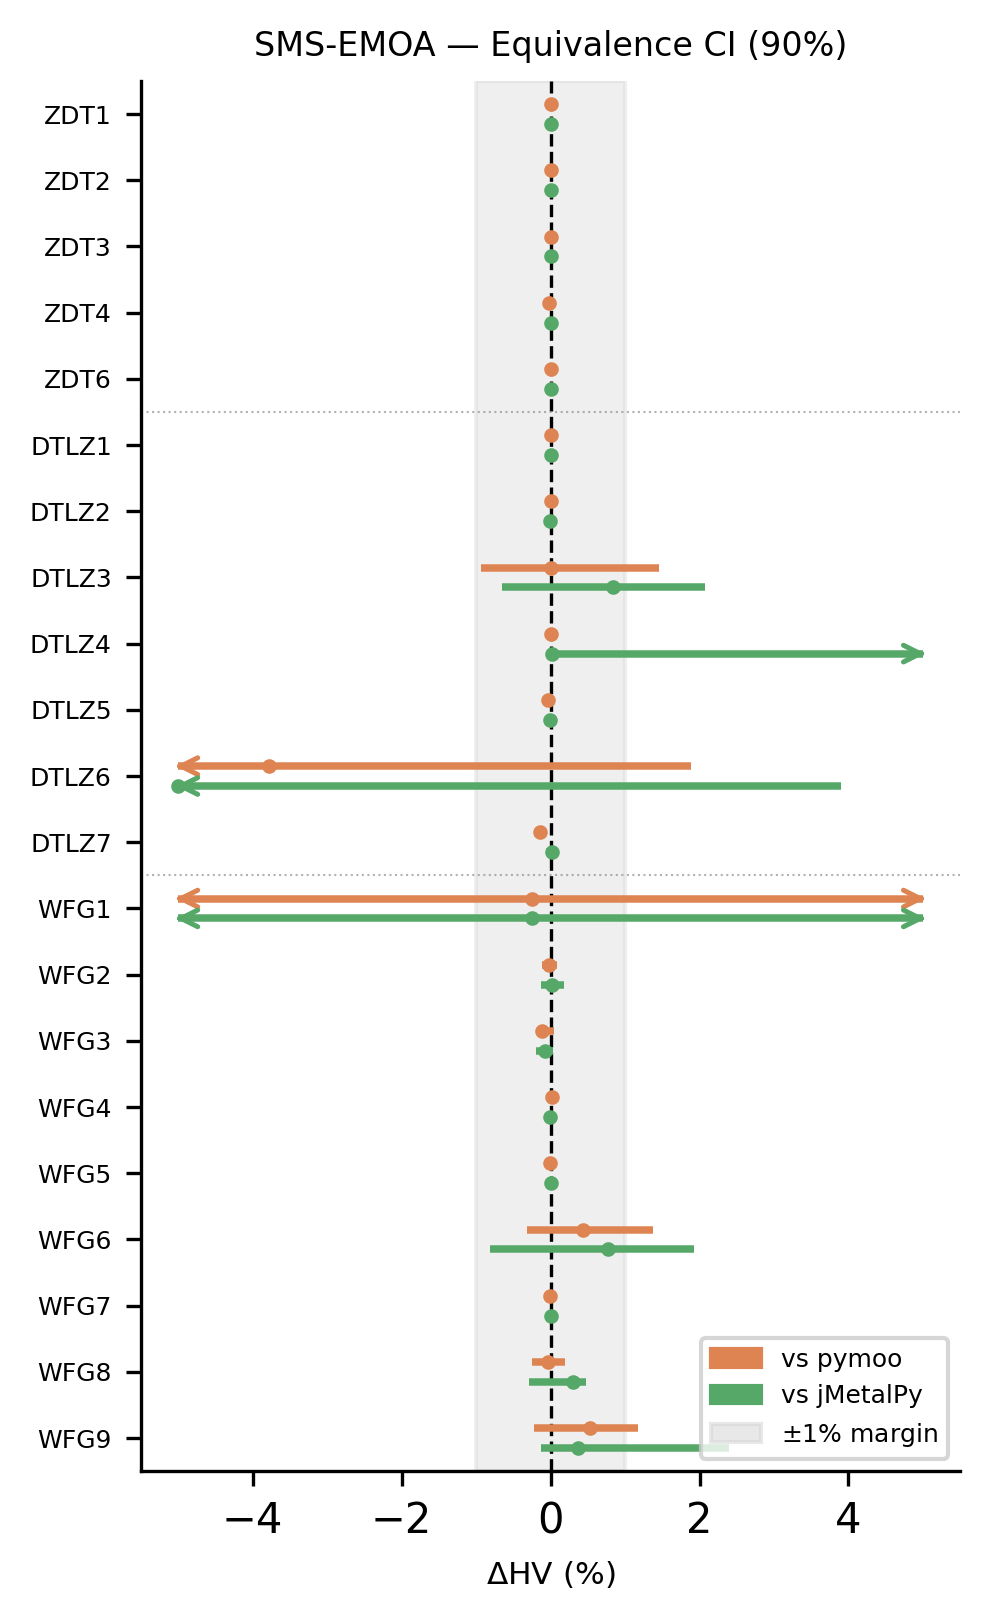
\includegraphics[width=\columnwidth]{forest_ci_smsemoa.png}
  \caption{SMS-EMOA. Per-problem paired bootstrap 90\% confidence intervals for the relative normalized hypervolume difference $\Delta = (\HV_{\text{\VAMOS}} - \HV_{\text{fw}})/\HV_{\text{fw}}$, reported in percent. The shaded band marks the $\pm 1\%$ equivalence margin; intervals falling entirely within this band indicate statistical equivalence}
  \label{fig:forest_ci_smsemoa}
\end{figure}
\endgroup

\subsection{MOEA/D}

Tables~\ref{tab:stats_hypervolume_moead}--\ref{tab:hv_robustness_summary_moead} and Fig.~\ref{fig:forest_ci_moead} present the corresponding analyses for MOEA/D.

\begingroup
\setlength{\tabcolsep}{2pt}
\begin{table}[htbp]
\centering
\caption{MOEA/D. Normalized hypervolume comparison with Wilcoxon signed-rank test results (Holm-corrected)}
\label{tab:stats_hypervolume_moead}
\begin{tabular}{lccccc}
\toprule
\textbf{Problem} & \textbf{VAMOS} & \textbf{pymoo} & \textbf{p-value} & \textbf{$\hat{A}_{12}$} & \textbf{Sig.} \\
\midrule
zdt1 & \textbf{0.993} & 0.992 & <0.0001 & 0.98 & \checkmark \\
zdt2 & \textbf{0.986} & 0.986 & 0.010 & 0.74 & \checkmark \\
zdt3 & \textbf{0.993} & 0.993 & <0.0001 & 1.00 & \checkmark \\
zdt4 & \textbf{1.001} & 1.001 & 1.000 & 0.60 &  \xmark \\
zdt6 & \textbf{0.987} & 0.985 & <0.0001 & 0.98 & \checkmark \\
dtlz1 & \textbf{0.901} & 0.862 & <0.0001 & 1.00 & \checkmark \\
dtlz2 & \textbf{0.832} & 0.795 & <0.0001 & 1.00 & \checkmark \\
dtlz3 & \textbf{0.809} & 0.790 & 0.308 & 0.74 &  \xmark \\
dtlz4 & \textbf{0.833} & 0.637 & 0.034 & 0.86 & \checkmark \\
dtlz5 & 0.952 & \textbf{0.952} & 1.000 & 0.50 &  \xmark \\
dtlz6 & \textbf{0.602} & 0.601 & 1.000 & 0.47 &  \xmark \\
dtlz7 & \textbf{0.666} & 0.650 & <0.0001 & 0.85 & \checkmark \\
wfg1 & 0.241 & \textbf{0.373} & <0.0001 & 0.11 & \checkmark \\
wfg2 & 1.005 & \textbf{1.006} & 1.000 & 0.49 &  \xmark \\
wfg3 & 0.977 & \textbf{0.978} & 0.121 & 0.27 &  \xmark \\
wfg4 & \textbf{0.967} & 0.965 & 0.033 & 0.76 & \checkmark \\
wfg5 & \textbf{0.828} & 0.828 & 0.059 & 0.81 &  \xmark \\
wfg6 & 0.837 & \textbf{0.838} & 1.000 & 0.49 &  \xmark \\
wfg7 & 0.971 & \textbf{0.972} & 0.452 & 0.37 &  \xmark \\
wfg8 & 0.759 & \textbf{0.762} & 1.000 & 0.43 &  \xmark \\
wfg9 & 0.928 & \textbf{0.929} & 1.000 & 0.55 &  \xmark \\
zcat1 & \textbf{0.983} & 0.983 & 1.000 & 0.66 &  \xmark \\
zcat2 & \textbf{0.988} & 0.987 & <0.0001 & 0.98 & \checkmark \\
zcat3 & \textbf{0.983} & 0.983 & 1.000 & 0.63 &  \xmark \\
zcat4 & \textbf{0.983} & 0.983 & 1.000 & 0.57 &  \xmark \\
zcat5 & \textbf{0.991} & 0.991 & <0.0001 & 0.98 & \checkmark \\
zcat6 & 0.995 & \textbf{0.995} & 1.000 & 0.44 &  \xmark \\
zcat7 & \textbf{0.983} & 0.983 & 1.000 & 0.64 &  \xmark \\
zcat8 & \textbf{0.968} & 0.968 & 0.682 & 0.69 &  \xmark \\
zcat9 & \textbf{0.968} & 0.968 & 1.000 & 0.58 &  \xmark \\
zcat10 & \textbf{0.934} & 0.934 & 1.000 & 0.66 &  \xmark \\
zcat11 & 0.986 & \textbf{0.986} & 1.000 & 0.48 &  \xmark \\
zcat12 & 0.986 & \textbf{0.986} & 1.000 & 0.39 &  \xmark \\
zcat13 & \textbf{1.010} & 1.009 & <0.0001 & 1.00 & \checkmark \\
zcat14 & \textbf{0.976} & 0.976 & 0.190 & 0.75 &  \xmark \\
zcat15 & 0.986 & \textbf{0.986} & 1.000 & 0.45 &  \xmark \\
zcat16 & 0.982 & \textbf{0.982} & 1.000 & 0.50 &  \xmark \\
zcat17 & \textbf{0.991} & 0.991 & <0.0001 & 0.97 & \checkmark \\
zcat18 & \textbf{0.983} & 0.983 & 1.000 & 0.66 &  \xmark \\
zcat19 & 0.985 & \textbf{0.985} & 1.000 & 0.43 &  \xmark \\
zcat20 & \textbf{0.983} & 0.983 & 1.000 & 0.60 &  \xmark \\
\bottomrule
\end{tabular}
\end{table}

\begin{table}[htbp]
\centering
\caption{MOEA/D. IGD+ comparison with Wilcoxon signed-rank test results (Holm-corrected). Lower is better}
\label{tab:stats_igd_plus_moead}
\begin{tabular}{lccccc}
\toprule
\textbf{Problem} & \textbf{VAMOS} & \textbf{pymoo} & \textbf{p-value} & \textbf{$\hat{A}_{12}$} & \textbf{Sig.} \\
\midrule
zdt1 & \textbf{0.0025} & 0.0025 & 0.000 & 0.18 & \checkmark \\
zdt2 & \textbf{0.0025} & 0.0025 & <0.0001 & 0.12 & \checkmark \\
zdt3 & \textbf{0.0026} & 0.0027 & <0.0001 & 0.00 & \checkmark \\
zdt4 & \textbf{0.0008} & 0.0009 & 0.467 & 0.36 &  \xmark \\
zdt6 & \textbf{0.0023} & 0.0026 & <0.0001 & 0.01 & \checkmark \\
dtlz1 & \textbf{0.0218} & 0.0235 & <0.0001 & 0.11 & \checkmark \\
dtlz2 & \textbf{0.0334} & 0.0344 & <0.0001 & 0.01 & \checkmark \\
dtlz3 & \textbf{0.0395} & 0.0396 & 1.000 & 0.46 &  \xmark \\
dtlz4 & \textbf{0.0345} & 0.1186 & 0.020 & 0.13 & \checkmark \\
dtlz5 & \textbf{0.0036} & 0.0036 & 1.000 & 0.43 &  \xmark \\
dtlz6 & \textbf{0.0698} & 0.0748 & 1.000 & 0.48 &  \xmark \\
dtlz7 & \textbf{0.0746} & 0.0790 & <0.0001 & 0.07 & \checkmark \\
wfg1 & 0.9082 & \textbf{0.7454} & <0.0001 & 0.87 & \checkmark \\
wfg2 & 0.2169 & \textbf{0.2163} & 1.000 & 0.49 &  \xmark \\
wfg3 & 0.0171 & \textbf{0.0152} & 0.026 & 0.76 & \checkmark \\
wfg4 & \textbf{0.0102} & 0.0104 & 1.000 & 0.44 &  \xmark \\
wfg5 & 0.0694 & \textbf{0.0690} & 0.002 & 0.79 & \checkmark \\
wfg6 & 0.0746 & \textbf{0.0682} & 1.000 & 0.49 &  \xmark \\
wfg7 & 0.0094 & \textbf{0.0082} & 0.001 & 0.80 & \checkmark \\
wfg8 & 0.1382 & \textbf{0.1336} & 0.147 & 0.69 &  \xmark \\
wfg9 & \textbf{0.0385} & 0.0399 & 0.311 & 0.41 &  \xmark \\
zcat1 & \textbf{0.0070} & 0.0071 & <0.0001 & 0.11 & \checkmark \\
zcat2 & \textbf{0.0064} & 0.0068 & <0.0001 & 0.00 & \checkmark \\
zcat3 & \textbf{0.0072} & 0.0073 & 0.000 & 0.16 & \checkmark \\
zcat4 & \textbf{0.0072} & 0.0073 & <0.0001 & 0.14 & \checkmark \\
zcat5 & \textbf{0.0053} & 0.0055 & <0.0001 & 0.01 & \checkmark \\
zcat6 & \textbf{0.0027} & 0.0028 & 0.100 & 0.21 &  \xmark \\
zcat7 & \textbf{0.0061} & 0.0062 & 0.147 & 0.25 &  \xmark \\
zcat8 & \textbf{0.0066} & 0.0069 & <0.0001 & 0.06 & \checkmark \\
zcat9 & \textbf{0.0067} & 0.0068 & 0.000 & 0.14 & \checkmark \\
zcat10 & \textbf{0.0045} & 0.0046 & <0.0001 & 0.09 & \checkmark \\
zcat11 & \textbf{0.0065} & 0.0066 & 0.001 & 0.19 & \checkmark \\
zcat12 & \textbf{0.0065} & 0.0067 & 0.004 & 0.16 & \checkmark \\
zcat13 & \textbf{0.0060} & 0.0064 & <0.0001 & 0.00 & \checkmark \\
zcat14 & \textbf{0.0076} & 0.0078 & <0.0001 & 0.08 & \checkmark \\
zcat15 & \textbf{0.0066} & 0.0066 & 0.147 & 0.26 &  \xmark \\
zcat16 & \textbf{0.0068} & 0.0068 & 0.000 & 0.16 & \checkmark \\
zcat17 & \textbf{0.0053} & 0.0054 & <0.0001 & 0.01 & \checkmark \\
zcat18 & \textbf{0.0062} & 0.0063 & 0.311 & 0.23 &  \xmark \\
zcat19 & \textbf{0.0062} & 0.0063 & 0.001 & 0.14 & \checkmark \\
zcat20 & \textbf{0.0062} & 0.0062 & 0.147 & 0.26 &  \xmark \\
\bottomrule
\end{tabular}
\end{table}

\begin{table}[htbp]
\centering
\caption{Normalized hypervolume equivalence summary (paired bootstrap 90\% CI; equivalence margin $\pm 1\%$ relative)}
\label{tab:hv_equivalence_summary_moead}
\begin{tabular}{lccc}
\toprule
\textbf{Framework} & \textbf{Eq.\ problems} & \textbf{Non-inf.\ problems} & \textbf{Median $\Delta$HV (\%)} \\
\midrule
\textit{pymoo} & 32/41 & 39/41 & +0.01 \\
\textit{jMetalPy} & 36/41 & 38/41 & +0.00 \\
\textit{Platypus} & 20/20 & 20/20 & +0.03 \\
\bottomrule
\end{tabular}
\end{table}

\begin{table}[htbp]
\centering
\caption{Robustness summary for normalized hypervolume across seeds (median across problems). ``Near-best'' is defined per problem as HV $\ge 0.99 \cdot \max$ median(HV) among frameworks}
\label{tab:hv_robustness_summary_moead}
\begin{tabular}{lcc}
\toprule
\textbf{Framework} & \textbf{Median IQR(HV)} & \textbf{Median \% seeds near-best} \\
\midrule
VAMOS & 0.000 & 100.0 \\
\textit{pymoo} & 0.000 & 100.0 \\
\textit{jMetalPy} & 0.000 & 100.0 \\
\textit{Platypus} & 0.000 & 100.0 \\
\bottomrule
\end{tabular}
\end{table}

\begin{figure}[htbp]
  \centering
  
\includegraphics[width=\columnwidth]{forest_ci_moead.png}
  \caption{MOEA/D. Per-problem paired bootstrap 90\% confidence intervals for the relative normalized hypervolume difference $\Delta = (\HV_{\text{\VAMOS}} - \HV_{\text{fw}})/\HV_{\text{fw}}$, reported in percent. The shaded band marks the $\pm 1\%$ equivalence margin; intervals falling entirely within this band indicate statistical equivalence}
  \label{fig:forest_ci_moead}
\end{figure}
\endgroup

%==============================================================================
\section{Accessibility Proxy Protocol}
\label{app:accessibility_protocol}
%==============================================================================

To complement the accessibility discussion in the main paper, we evaluate three onboarding tasks: (i)~run NSGA-II on a built-in benchmark, (ii)~define and optimize a small custom two-objective problem, and (iii)~move from defaults to explicit operator-level configuration. For each framework, we selected a canonical snippet from the shortest documented path available in March~2026. For \VAMOS{}, the snippets align with the public API examples used in the manuscript; for \textit{pymoo}  and jMetalPy, the canonical sources are the public documentation pages listed in Table~\ref{tab:accessibility_proxy_details}.

Metrics count only non-empty, non-comment lines and explicit \texttt{import}/\texttt{from} statements. Plotting, result serialization, and explanatory comments are excluded because they do not affect the onboarding burden of the optimization call itself. The underlying artifact file used to generate the accessibility-proxy table in the main paper and Table~\ref{tab:accessibility_proxy_details} below is \texttt{paper/accessibility\_proxy\_snippets.json}.

\begin{table*}[htbp]
\centering
\scriptsize
\setlength{\tabcolsep}{4pt}
\caption{Detailed accessibility-proxy artifacts used in the manuscript. LOC counts non-empty, non-comment lines in the canonical snippet; imports counts explicit \texttt{import}/\texttt{from} statements.}
\label{tab:accessibility_proxy_details}
\begin{tabular}{@{}llcccp{0.53\textwidth}@{}}
\toprule
\textbf{Task} & \textbf{Framework} & \textbf{LOC} & \textbf{Imports} & \textbf{Entry} & \textbf{Canonical source} \\
\midrule
Built-in run & VAMOS & 2 & 1 & \texttt{optimize(...)} & \texttt{examples/basics/quickstart.py} \\
Built-in run & pymoo & 6 & 3 & \texttt{minimize(...)} & pymoo NSGA-II docs (\url{https://pymoo.org/algorithms/moo/nsga2.html}) \\
Built-in run & jMetalPy & 6 & 2 & \texttt{algorithm.run()} & jMetalPy index quick example (\url{https://jmetal.github.io/jMetalPy/index.html}) \\
\midrule
Custom problem & VAMOS & 11 & 1 & \texttt{optimize(...)} & \texttt{paper/manuscript/main.tex} \\
Custom problem & pymoo & 12 & 4 & \texttt{minimize(...)} & pymoo FunctionalProblem docs (\url{https://pymoo.org/problems/definition.html}) \\
Custom problem & jMetalPy & 22 & 5 & \texttt{algorithm.run()} & jMetalPy OnTheFlyFloatProblem docs (\url{https://jmetal.github.io/jMetalPy/tutorials/problem.html}) \\
\midrule
Expert config & VAMOS & 16 & 2 & \texttt{optimize(...)} & \texttt{paper/manuscript/main.tex} \\
Expert config & pymoo & 13 & 5 & \texttt{minimize(...)} & pymoo NSGA-II docs (\url{https://pymoo.org/algorithms/moo/nsga2.html}) \\
Expert config & jMetalPy & 17 & 5 & \texttt{algorithm.run()} & jMetalPy getting started (\url{https://jmetal.github.io/jMetalPy/getting-started.html}) \\
\bottomrule
\end{tabular}
\end{table*}


%==============================================================================
\section{Code Examples}
\label{app:code}
%==============================================================================

Representative code examples and tuning scripts will be made available upon acceptance.


%==============================================================================
\section{Parameter Spaces for pymoo and jMetalPy}
\label{app:parameter_spaces}
%==============================================================================

Tables~\ref{tab:parameter_space_pymoo} and~\ref{tab:parameter_space_jmetalpy} detail the configurable parameter spaces for NSGA-II in \textit{pymoo} and \textit{jMetalPy}, respectively.

\begin{table*}[htbp]
\centering
\caption{Parameter space for NSGA-II in \textit{pymoo}  (real-valued encoding). Parameters in italics are conditional, active only when their corresponding operator is selected. Values in \textbf{bold} indicate defaults. The total number of configurable parameters is 20 (11 always active, 9~conditional). Acronyms in the table denote Latin hypercube sampling (LHS), parent-centric crossover (PCX), and differential evolution crossover (DEX).}
\label{tab:parameter_space_pymoo}
\resizebox{\textwidth}{!}{%
\begin{tabular}{lll}
\toprule
\textbf{Component} & \textbf{Value / Strategy} & \textbf{Conditional Parameters} \\ \midrule
\multirow{2}{*}{General} & Pop.\ Size: integer; default $\mathbf{100}$ & -- \\
 & Offspring Count (\texttt{n\_offsprings}): integer; default = Pop.\ Size & -- \\ \midrule
\multirow{1}{*}{Initialization} & \{\textbf{Random}, LHS\} & -- \\ \midrule
\multirow{3}{*}{Selection} & \{\textbf{Tournament}, Random\} & -- \\
 & \textit{Tournament Size} (\texttt{pressure}): integer; default $\mathbf{2}$ & \textit{Selection} = Tournament \\
 & Crowding Metric $\in$ \{\textbf{cd}, pcd, ce, mnn, 2nn\} & -- \\ \midrule
\multirow{4}{*}{Crossover} & \multicolumn{2}{l}{\textit{Global:} Probability $\in \Realdomain{0, 1}$; default $\mathbf{0.9}$} \\
 & \textbf{SBX} & \textit{Dist.\ Index} $\eta \in \Realdomain{3, 30}$; default $\mathbf{15}$. \textit{Per-var.\ prob.}\ $\in \Realdomain{0.1, 0.9}$; default $\mathbf{0.5}$ \\
 & PCX & $\eta \in \Realdomain{0.01, 0.3}$, $\zeta \in \Realdomain{0.01, 0.3}$ \\
 & DEX & $CR \in \Realdomain{0, 1}$; default $0.7$. $F$: real or \texttt{None} \\ \midrule
\multirow{3}{*}{Mutation} & \multicolumn{2}{l}{\textit{Global:} Prob.\ $\in \Realdomain{0, 1}$; default $\mathbf{0.9}$. Per-var.\ prob.; default $\min(0.5, 1/n)$} \\
 & \textbf{Polynomial} & \textit{Dist.\ Index} $\eta \in \Realdomain{3, 30}$; default $\mathbf{20}$ \\
 & Gaussian & $\sigma \in \Realdomain{0.01, 0.25}$; default $0.1$ \\ \midrule
\multirow{1}{*}{Repair} & \{\textbf{clip}, bounce-back, to-bound\} & -- \\ \bottomrule
\end{tabular}%
}
\end{table*}

\begin{table*}[htbp]
\centering
\caption{Parameter space for NSGA-II in \textit{jMetalPy} (real-valued encoding). Parameters in italics are conditional, active only when their corresponding operator is selected. Values in \textbf{bold} indicate defaults. The total number of configurable parameters is 29 (10 always active, 19~conditional). Acronyms in the table denote unimodal normal distribution crossover (UNDX) and differential evolution (DE).}
\label{tab:parameter_space_jmetalpy}
%\resizebox{\textwidth}{!}{%
\begin{tabular}{lll}
\toprule
\textbf{Component} & \textbf{Value / Strategy} & \textbf{Conditional Parameters} \\ \midrule
\multirow{5}{*}{General} & Pop.\ Size: integer & -- \\
 & Offspring Pop.\ Size: integer; $= 1$ for steady-state & -- \\
 & Use External Archive $\in$ \{True, \textbf{False}\} & -- \\
 & \textit{Archive Type} $\in$ \{NonDominated, CrowdingDist., DistanceBased\} & \textit{Archive} = True \\
 & \textit{Archive Max Size}: integer & \textit{Archive} = True, bounded \\ \midrule
\multirow{1}{*}{Initialization} & \{\textbf{Random}, Injector\} & -- \\ \midrule
\multirow{2}{*}{Selection} & \{\textbf{Binary Tournament}, Tournament, Random\} & -- \\
 & \textit{Tournament Size}: integer $\geq 2$ & \textit{Selection} = Tournament \\ \midrule
\multirow{7}{*}{Crossover} & \multicolumn{2}{l}{\textit{Global:} Probability $\in \Realdomain{0, 1}$} \\
 & \textbf{SBX} & \textit{Dist.\ Index}; default $\mathbf{20}$ \\
 & BLX-$\alpha$ & $\alpha$; default $0.5$ \\
 & BLX-$\alpha\beta$ & $\alpha$, $\beta$; default $0.5$ each \\
 & Arithmetic & -- \\
 & UNDX & $\zeta$; default $0.5$. $\eta$; default $0.35$ \\
 & DE & $CR \in \Realdomain{0, 1}$, $F \in \Realdomain{0, 2}$, $K \in \Realdomain{0, 1}$ \\ \midrule
\multirow{7}{*}{Mutation} & \multicolumn{2}{l}{\textit{Global:} Probability $\in \Realdomain{0, 1}$; conventionally $1/n$} \\
 & \textbf{Polynomial} & \textit{Dist.\ Index}; default $\mathbf{20}$ \\
 & Simple Random & -- \\
 & Uniform & \textit{Perturbation}; default $0.5$ \\
 & Non-Uniform & \textit{Perturbation}, \textit{Max Iterations} \\
 & L\'evy Flight & $\beta$; default $1.5$. \textit{Step size}; default $0.01$ \\
 & Power Law & $\delta$; default $1.0$ \\ \midrule
\multirow{1}{*}{Repair} & \{\textbf{Clamp}, Random Uniform, Reflective, Bound Swap\} & -- \\ \bottomrule
\end{tabular}%
%}
\end{table*}

%==============================================================================
% Bibliography
%==============================================================================
\bibliographystyle{IEEEtran}
\bibliography{references}

\end{document}
